\documentclass{article}

\usepackage{blindtext}
\usepackage{geometry}
\geometry{
    a4paper,
    total={170mm,257mm},
    left=25mm,
    right=25mm,
    top=15mm,
}
\usepackage{graphicx}
\usepackage{amsmath,amsthm,amssymb}
\usepackage{nccmath}
\usepackage{mathtext}
\usepackage[T1,T2A]{fontenc}
\usepackage[utf8]{inputenc}
\usepackage[russian]{babel}

\setlength{\parindent}{0mm}

\title{
\textit{\small{Georgii Potoshin, 2023}}\\
\vspace{0.3ex}
\textit{\huge{Leçon de potions}}\vspace{1ex}
}

\date{\vspace{-8ex}}

\begin{document}
\maketitle
\begin{center}
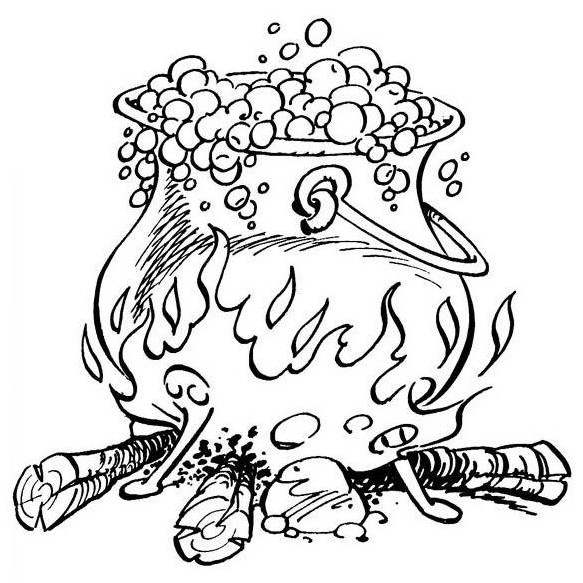
\includegraphics[scale=0.5]{cotel.jpeg}
\end{center}
\begin{center}\textsc{\Large{Élixir n° 1 - Potion d'Allégresse}}\end{center}
\begin{enumerate}
    \item
		Un pot de Potion d'Allégresse nécessite 1 tasse d'yeux d'escargot, 2
		tasses d'écailles de dragon et 3 tasses d'eau. Combien de tasses
		d'écailles de dragon faut-il prendre pour faire une chaudière de Potion
		d'Allégresse si la chaudière contient 3 pots ?
	\item
		Vous avez deux sabliers. L'un mesure 3 minutes et l'autre 10 minutes.
		La Potion d'Allégresse doit être infusée pendant exactement 16 minutes. 
		Comment la préparez-vous ?
	\item
		Vous avez maintenant un chaudron de douze litres de Potion d'Allégresse.
		Mais vous n'avez besoin que de six litres. Vous avez des petits
		chaudrons de 8 litres et de 5 litres, mais pas d'instruments 
		de mesure (et les pots ont tous disparu). Comment verser 6 litres de 
		potion dans un chaudron de 8 litres ?
\end{enumerate}
\vspace{1ex}
\begin{center}\textsc{\Large{Élixir n° 2 - Potion de Chance}}\end{center}
\begin{enumerate}
	\item
		Pour obtenir 9 verres de Potion de Chance, il faut 2 verres de plumes
		de corbeau, 3 verres d'extrait de limaces, 1 verre de cils de dragon et
		3 verres d'eau. Combien de verres d'extrait de limaces faut-il prendre
		pour obtenir 21 verres de Potion ?
	\item
		Vous avez les mêmes sabliers de 3 et 10 minutes. Il faut faire bouillir
		la Potion de Chance exactement pendant 7 minutes. Comment pouvez-vous
		le faire ?
	\item
		Vous avez 21 litres de Potion de Chance dans une grande marmite. Vous
		avez besoin de 5 litres. Cependant, vous n'avez que des petites 
		chaudrons de 3 et 7 litres. Comment pouvez-vous transvaser 5 litres de
		potion dans le chaudrons de 7 litres ?
\end{enumerate}
\vspace{1ex}
\begin{center}\textsc{\Large{Élixir n°3 - Infusion d'Argousier}}\end{center}
\begin{enumerate}
	\item
		Pour préparer l'Infusion d'Argousier, vous devez ajouter 2 verres de
		pattes de grenouille, 3 verres de champignons séchés, 1 verre de baies
		de loup, 5 verres d'argousier et 4 parts d'eau. Combien de verres de
		champignons séchés devez-vous prendre pour obtenir 30 verres d'élixir ?
	\item
		Vous disposez de deux sabliers, l'un pour 3 minutes et l'autre pour 10
		minutes. Il est nécessaire de faire bouillir l'Infusion d'Argousier
		pendant exactement 4 minutes. Comment allez-vous procéder ?
	\item
		Vous avez 8 litres d'Infusion d'Argousier. Vous disposez également de
		deux petites casseroles de 2 et 3 litres. Comment mesurer précisément 4
		litres ? Attention : si vous faites plus de trois transvasements,
		l'élixir décidera de détruire tout votre laboratoire !
\end{enumerate}
\vspace{1ex}
\begin{center}\textsc{\Large{Élixir n°4 - Potion du Phoenix}}\end{center}
\begin{enumerate}
	\item
		Dans le four de laboratoire se trouve une chaudière où bouillonnent 9
		litres de lave. Dans le processus de fabrication de la Potion du
		Phénix, il est nécessaire d'ajouter à la chaudière 3 litres de lave à
		intervalles réguliers, à trois reprises. Comment réaliser cela si l'on
		dispose uniquement de trois récipients ignifuges d'une capacité de 5, 4
		et 2 litres ? (Autrement dit, il faut obtenir 3 portions de 3 litres
		chacune.)
	\item 
		Après l'ajout des derniers 3 litres d'étain, il faut faire bouillir
		l'Elixir du Phénix pendant exactement 5 minutes. Comment pouvez-vous le
		faire si vous disposez toujours de deux sabliers, l'un de 3 minutes et
		l'autre de 10 minutes ?
\end{enumerate}
\end{document}
